\section{The legality study}\label{old:9}

\textbf{Question.} Can a policy trained \emph{without} the mask learn the rules well enough to play legally on its own? Does that cost or gain playing strength compared with Maskable PPO, and which objective (\S\ref{old:5}) gets there? Setup: \S\ref{old:6.4}. Protocol: \S\ref{old:7}.

\textbf{Which rules.} Every number in this section was measured in \code{TnGEnv} before the capture correction of Section~\ref{sec:rulefix}, the rule under which all these models were trained. Section~\ref{sec:cmp-fix} repeats the comparison under the corrected rule; the conclusions about legality do not depend on it.

\subsection{Final models, tanh (1,000 games per cell)}\label{old:9.1}

$W$ is the goat win rate against each tiger. $\bar P^{\text{ill}}_0, \bar P^{\text{ill}}_1$ are the illegal probabilities in the placement and movement phases (\S\ref{old:7}).

{\footnotesize
\begin{longtable}{@{}>{\raggedright\arraybackslash}p{\dimexpr 0.275\linewidth-2\tabcolsep\relax}>{\raggedleft\arraybackslash}p{\dimexpr 0.122\linewidth-2\tabcolsep\relax}>{\raggedleft\arraybackslash}p{\dimexpr 0.115\linewidth-2\tabcolsep\relax}>{\raggedleft\arraybackslash}p{\dimexpr 0.099\linewidth-2\tabcolsep\relax}>{\raggedleft\arraybackslash}p{\dimexpr 0.092\linewidth-2\tabcolsep\relax}>{\raggedleft\arraybackslash}p{\dimexpr 0.053\linewidth-2\tabcolsep\relax}>{\raggedleft\arraybackslash}p{\dimexpr 0.053\linewidth-2\tabcolsep\relax}>{\raggedleft\arraybackslash}p{\dimexpr 0.191\linewidth-2\tabcolsep\relax}@{}}
\toprule
\textbf{Model} & \textbf{$W$ masked, greedy} & \textbf{$W$ masked, smart} & \textbf{$W$ raw, greedy} & \textbf{$W$ raw, smart} & \textbf{$\bar P^{\text{ill}}_0$} & \textbf{$\bar P^{\text{ill}}_1$} & \textbf{Raw games ended illegally} \\
\midrule
\endhead
Maskable PPO, seed 42 & 0.692 & 0.599 & 0 & 0 & 0.778 & 0.876 & 100\% \\
Maskable PPO, seed 7 & 0.718 & 0.619 & 0 & 0 & 0.790 & 0.805 & 100\% \\
PPO, no legality loss, seed 42 & 0.530 & 0 & 0.525 & 0 & 0.549 & 0.881 & 73.8\% \\
PPO, no legality loss, seed 7 & 0.637 & 0 & 0.576 & 0 & 0.448 & 0.870 & 71.2\% \\
\textbf{PPO + nll 0.5, seed 42} & \textbf{0.754} & \textbf{0.947} & \textbf{0.752} & \textbf{0.947} & 0.0010 & 0.029 & 3.6\% \\
PPO + nll 0.5, seed 7 & 0.547 & 0.023 & 0.536 & 0.023 & 0.0034 & 0.062 & 23.4\% \\
PPO + nll 2, seed 42 & 0.714 & 0.795 & 0.714 & 0.795 & \textbf{0.0002} & \textbf{0.0015} & \textbf{0.1\%} \\
PPO + mass 0.5 & 0.006 & 0 & 0.006 & 0 & 0.0007 & 0.504 & 99.6\% \\
KL penalty + nll 0.5 & 0.566 & 0.445 & 0.564 & 0.445 & 0.0030 & 0.069 & 7.6\% \\
SPO + nll 0.5 & 0.005 & 0 & 0.005 & 0 & 0.0023 & 0.179 & 97.4\% \\
clip + nll 0.5 + Huber & 0.628 & 0.336 & 0.627 & 0.336 & 0.0015 & 0.018 & 1.5\% \\
\emph{shipped NormalGoat (100M, greedy)} & 0.796 & 0.016 & 0 & 0 & 0.977 & 0.973 & 100\% \\
\emph{shipped SmartGoat (100M, smart)} & 0.067 & 0.944 & 0 & 0 & 0.844 & 0.992 & 100\% \\
\emph{shipped RobustGoat (60M, curriculum)} & 0.798 & 0.857 & 0 & 0 & 0.984 & 0.990 & 100\% \\
\bottomrule
\end{longtable}\addtocounter{table}{-1}
}

The raw lose-a-turn win rates equal the raw win rates to three decimals for every model, so the table omits them.

\subsection{Training dynamics (TensorBoard, last \textasciitilde{}40k steps of each run)}\label{old:9.2}

{\small
\begin{longtable}{@{}>{\raggedright\arraybackslash}p{\dimexpr 0.231\linewidth-2\tabcolsep\relax}>{\raggedleft\arraybackslash}p{\dimexpr 0.167\linewidth-2\tabcolsep\relax}>{\raggedleft\arraybackslash}p{\dimexpr 0.222\linewidth-2\tabcolsep\relax}>{\raggedleft\arraybackslash}p{\dimexpr 0.157\linewidth-2\tabcolsep\relax}>{\raggedleft\arraybackslash}p{\dimexpr 0.222\linewidth-2\tabcolsep\relax}@{}}
\toprule
\textbf{Run} & \textbf{\code{train/illegal\_\allowbreak{}prob}} & \textbf{Illegal endings (window)} & \textbf{Win rate (window)} & \textbf{Win rate first ≥ 0.10 at} \\
\midrule
\endhead
Maskable PPO (42 / 7) & — & 0 / 0 & 0.567 / 0.594 & 0.49M / 0.57M \\
no legality loss (42 / 7) & 0.119 / 0.114 & 0.756 / 0.750 & 0.244 / 0.250 & 1.39M / 1.72M \\
nll 0.5 (42 / 7) & 0.004 / 0.020 & 0.084 / 0.440 & 0.798 / 0.152 & 5.00M / 9.26M \\
nll 2 & 0.000 & 0.005 & 0.680 & 3.77M \\
mass 0.5 & 0.049 & 0.999 & 0.001 & never \\
KL penalty + nll 0.5 & 0.022 & 0.489 & 0.163 & 9.34M \\
SPO + nll 0.5 & 0.042 & 0.877 & 0.000 & never \\
clip + nll 0.5 + Huber & 0.006 & 0.119 & 0.324 & 5.98M \\
\bottomrule
\end{longtable}\addtocounter{table}{-1}
}


\begin{figure}[H]
\centering
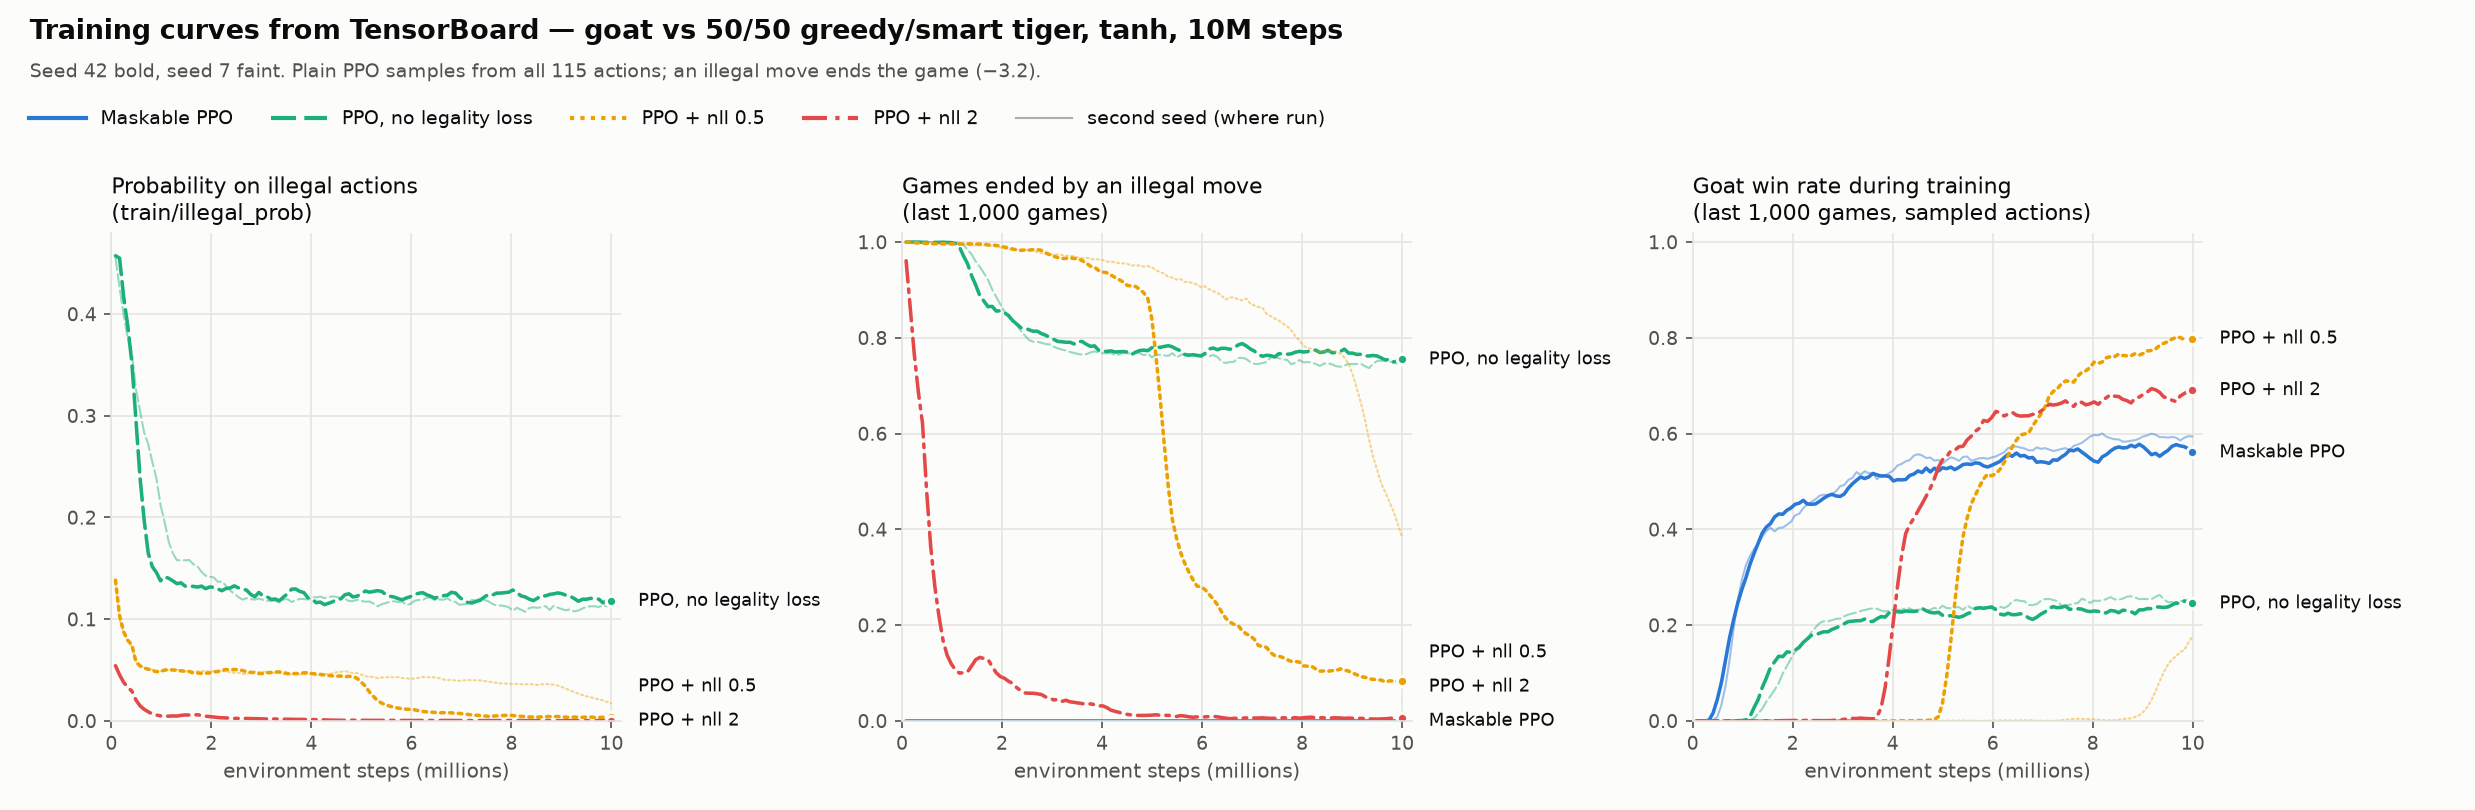
\includegraphics[width=0.98\linewidth]{figures/1_training_curves.png}
\caption{Training curves of the tanh runs of the legality study (TensorBoard).}\label{fig:curves}
\end{figure}

\begin{figure}[H]
\centering
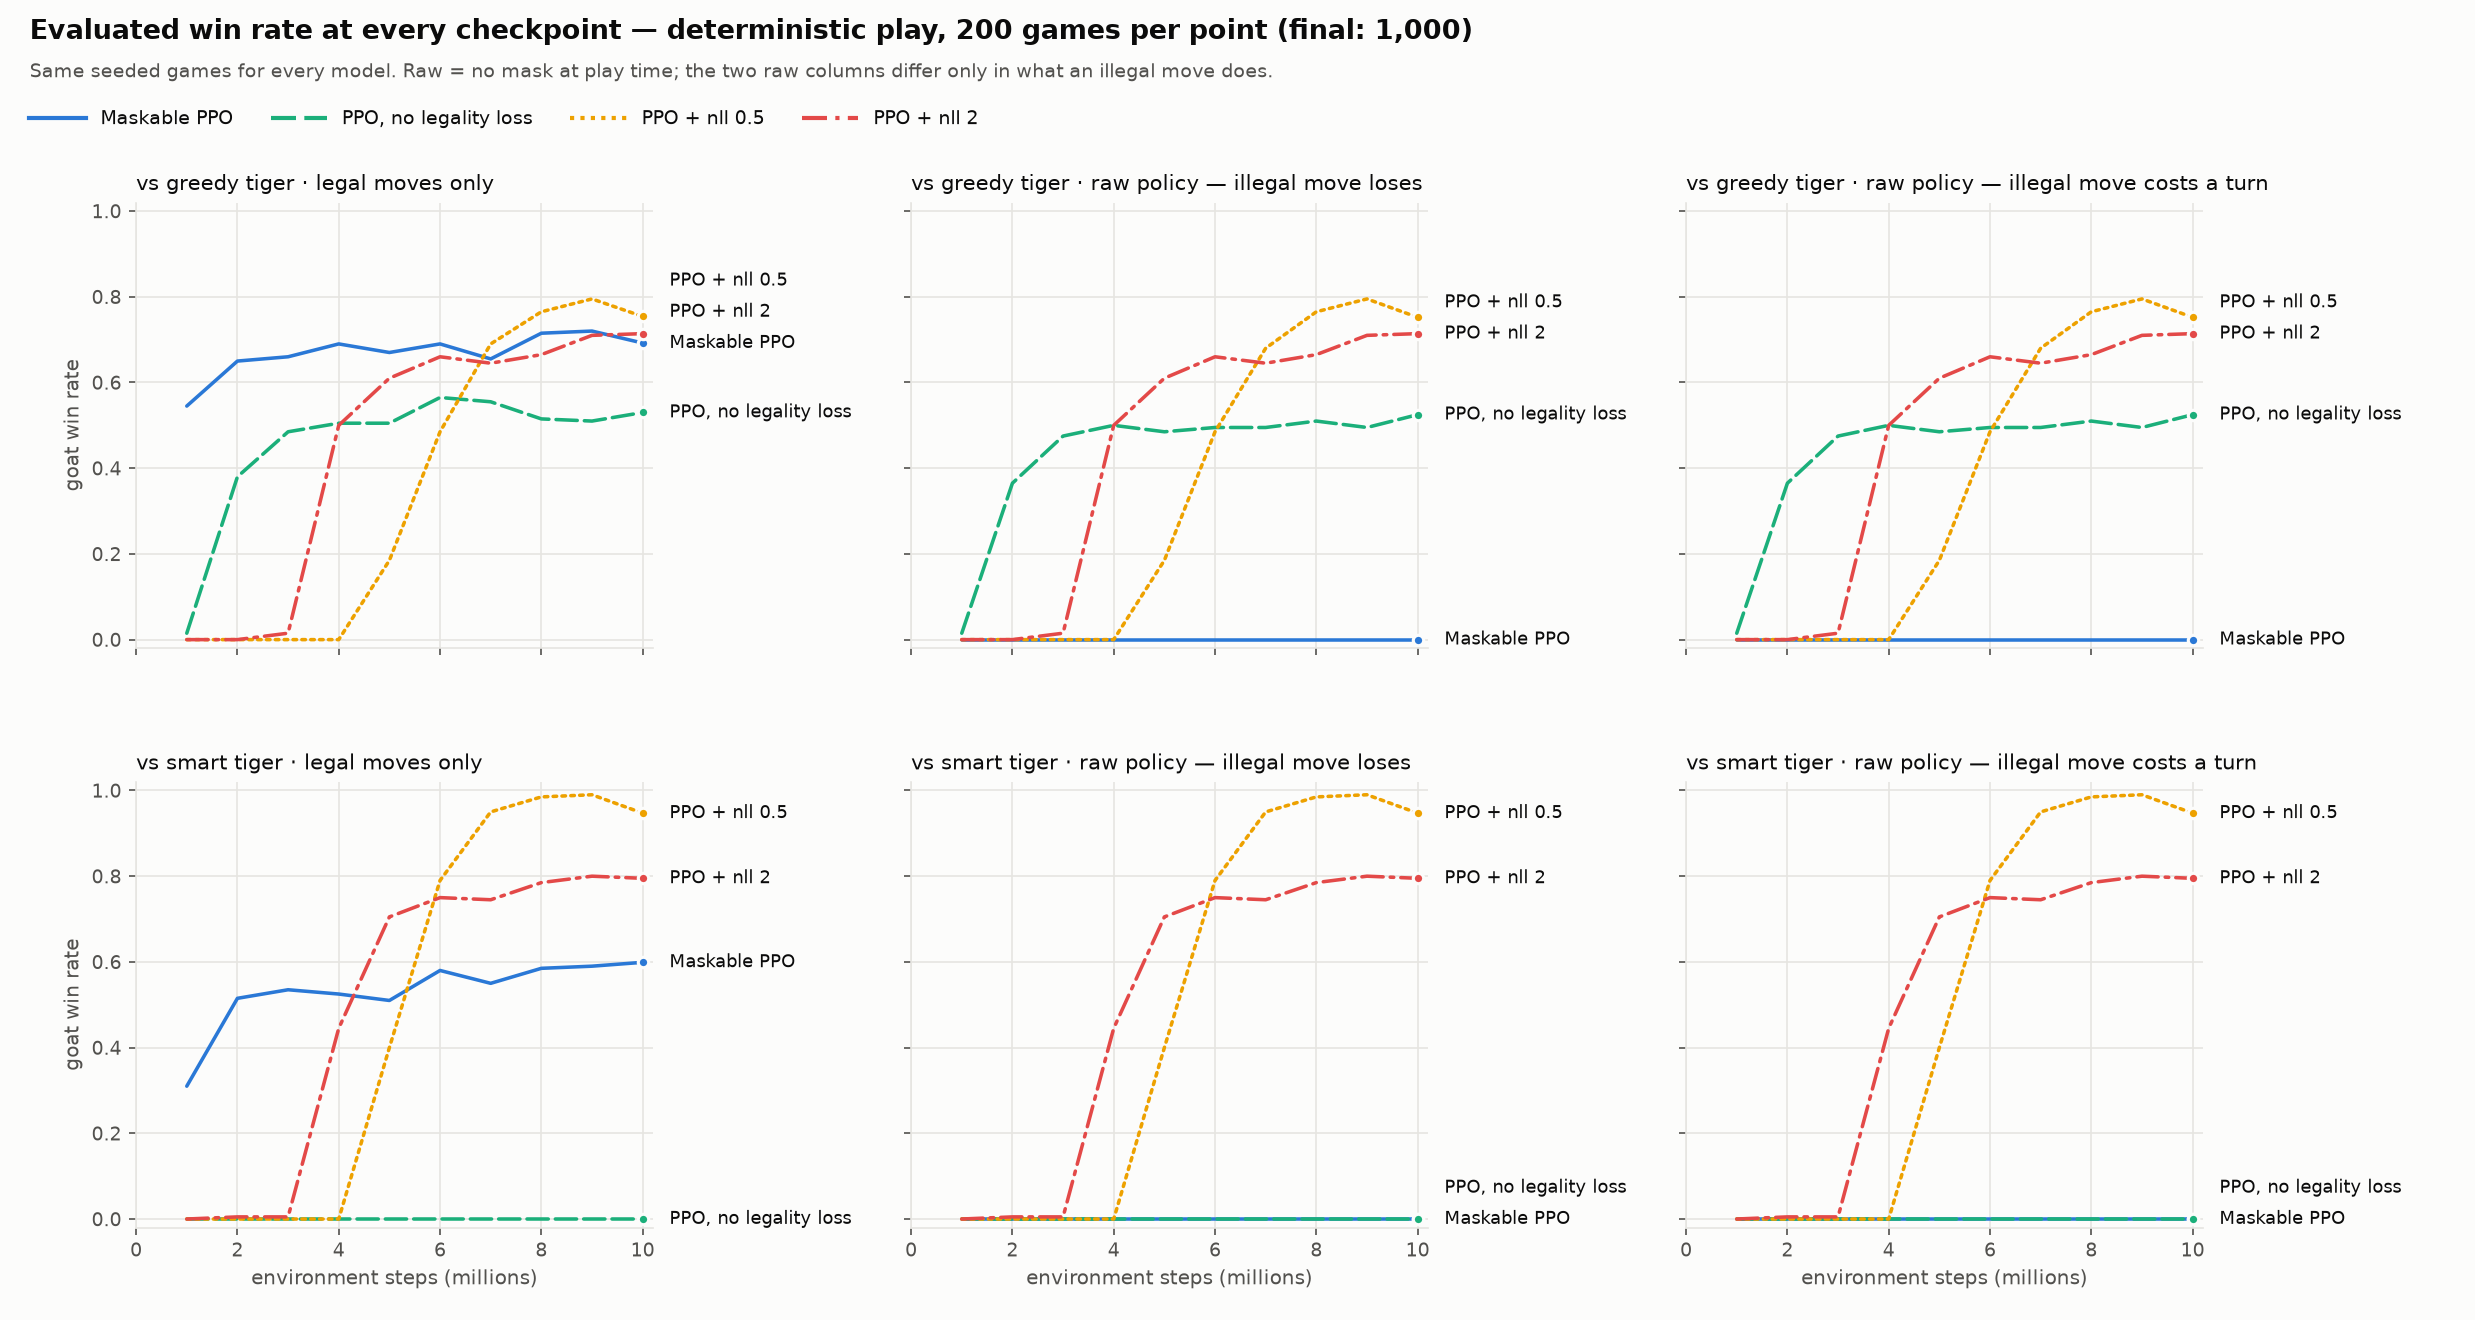
\includegraphics[width=0.98\linewidth]{figures/2_checkpoint_eval.png}
\caption{Checkpoint evaluations every 1M steps (200 games per point).}\label{fig:ckpt}
\end{figure}

\subsection{Findings}\label{old:9.3}

\begin{enumerate}
\item \textbf{Masking teaches the network nothing about legality.} After 10M steps, Maskable PPO still puts 78–88\% of its raw probability on illegal actions. The shipped models put 84–99\% there after 60–100M steps. Without the mask they lose every game. This is the zero-gradient property of \S\ref{old:3.2}: no loss term ever touches an illegal logit.
\item \textbf{The reward alone teaches legality only partly.} Plain PPO with $c_{\text{legal}} = 0$ learns to avoid most illegal moves in deterministic play (53–58\% raw wins against greedy). But it keeps 11–12\% illegal probability on its training states, and 71–74\% of its raw games still end in an illegal move. It never beats the smart tiger.
\item \textbf{The \code{nll} legality loss gives fully legal play and, for seed 42, the strongest goat in the study.} With $c_{\text{legal}} = 0.5$ (seed 42), masked and raw win rates agree to 0.002. Of its 3.6\% illegal raw endings, at most 2 in 2,000 games are games it wins with the mask. Against the smart tiger it wins 94.7\%, against 59.9\% for Maskable PPO at the same budget and 85.7\% for the 60M-step RobustGoat. With $c_{\text{legal}} = 2$ the network is almost perfectly legal ($\bar P^{\text{ill}}_1 = 0.0015$) and still strong (71.4\% / 79.5\%).
\item \textbf{Training under ``end\_game'' has a long plateau, then a sharp take-off.} An illegal move ends the episode, so a winning game needs every move to be legal. With per-move illegal probability $p$, the chance of playing $n$ moves without one is $(1-p)^n$. At $p \approx 0.05$ and $n \approx 25$ moves, that is about 0.28, and the agent almost never reaches the movement phase. The \code{nll} term pushes $p$ down until play survives long enough for winning rewards to appear. The take-off then comes at 3.8M ($c_{\text{legal}} = 2$), 5.0M or 9.3M (two seeds of 0.5). The onset time is very seed-sensitive, which is why seed 7 of \code{nll} 0.5 ends far behind seed 42.
\item \textbf{\code{mass} fails, as \S\ref{old:5.4} predicts.} Its gradient on an illegal logit is $\pi(a \mid s)\,P_{\mathcal{L}}(s)$, which is tiny while $P_{\mathcal{L}}$ is tiny. It cleans up the placement phase ($\bar P^{\text{ill}}_0 = 0.0007$) but leaves half the movement-phase probability illegal, and 99.6\% of games end illegally.
\item \textbf{The policy loss matters.} With the same legality term, SPO never took off and KL penalty took off only at 9.3M. Huber took off at 6M and finished weaker than plain MSE. These are single seeds, and finding 4 shows how much the onset time varies between seeds. So these rank orders are suggestive, not established.
\end{enumerate}
\textbf{Limitations.}

\begin{itemize}
\item Most variants have one seed.
\item Evaluation uses the training opponents (greedy and smart).
\item The shipped models were trained on an earlier environment version (\S\ref{old:6.2}).
\item Win rate is measured with deterministic play only.
\end{itemize}
\subsection{ReLU vs tanh}\label{old:9.4}

Same settings and seed as \S\ref{old:9.1}, with $\operatorname{act} = $ ReLU (\S\ref{old:3.1}). 1,000 games per cell (Figure~\ref{fig:relu}).

{\footnotesize
\begin{longtable}{@{}>{\raggedright\arraybackslash}p{\dimexpr 0.382\linewidth-2\tabcolsep\relax}>{\raggedright\arraybackslash}p{\dimexpr 0.049\linewidth-2\tabcolsep\relax}>{\raggedleft\arraybackslash}p{\dimexpr 0.130\linewidth-2\tabcolsep\relax}>{\raggedleft\arraybackslash}p{\dimexpr 0.122\linewidth-2\tabcolsep\relax}>{\raggedleft\arraybackslash}p{\dimexpr 0.106\linewidth-2\tabcolsep\relax}>{\raggedleft\arraybackslash}p{\dimexpr 0.098\linewidth-2\tabcolsep\relax}>{\raggedleft\arraybackslash}p{\dimexpr 0.057\linewidth-2\tabcolsep\relax}>{\raggedleft\arraybackslash}p{\dimexpr 0.057\linewidth-2\tabcolsep\relax}@{}}
\toprule
\textbf{Model} & \textbf{act} & \textbf{$W$ masked, greedy} & \textbf{$W$ masked, smart} & \textbf{$W$ raw, greedy} & \textbf{$W$ raw, smart} & \textbf{$\bar P^{\text{ill}}_0$} & \textbf{$\bar P^{\text{ill}}_1$} \\
\midrule
\endhead
Maskable PPO & tanh & 0.692 & 0.599 & 0 & 0 & 0.778 & 0.876 \\
Maskable PPO & ReLU & \textbf{0.854} & \textbf{0.856} & 0 & 0 & 0.924 & 0.887 \\
PPO, no legality loss & tanh & 0.530 & 0 & 0.525 & 0 & 0.549 & 0.881 \\
PPO, no legality loss & ReLU & 0.008 & 0 & 0.002 & 0 & 0.010 & 0.843 \\
PPO + nll 0.5 & tanh & 0.754 & 0.947 & 0.752 & 0.947 & 0.0010 & 0.029 \\
PPO + nll 0.5 & ReLU & 0.662 & 0.743 & 0.660 & 0.743 & 0.0010 & 0.0084 \\
PPO + nll 2 & tanh & 0.714 & 0.795 & 0.714 & 0.795 & 0.0002 & 0.0015 \\
PPO + nll 2 & ReLU & 0.694 & 0.851 & 0.692 & 0.851 & 0.0001 & 0.0010 \\
KL penalty + nll 0.5 & tanh & 0.566 & 0.445 & 0.564 & 0.445 & 0.0030 & 0.069 \\
KL penalty + nll 0.5 & ReLU & 0.592 & 0 & 0.588 & 0 & 0.0035 & 0.066 \\
SPO + nll 0.5 & tanh & 0.005 & 0 & 0.005 & 0 & 0.0023 & 0.179 \\
SPO + nll 0.5 & ReLU & 0.009 & 0 & 0.009 & 0 & 0.0044 & 0.169 \\
PPO, no legality loss, lose a turn ($r_{\text{ill}} = -1$) & ReLU & 0.186 & 0.906 & 0.185 & 0.906 & 0.019 & 0.070 \\
PPO + nll 2, lose a turn ($r_{\text{ill}} = -1$) & ReLU & 0.011 & 0 & 0.011 & 0 & 0.0003 & 0.0026 \\
\bottomrule
\end{longtable}\addtocounter{table}{-1}
}

Findings (one seed per cell, so differences within about the seed spread of \S\ref{old:9.1} are not significant):

\begin{enumerate}
\item ReLU helps Maskable PPO the most: it becomes the strongest player under the mask (0.854 / 0.856), but it still needs the mask ($\bar P^{\text{ill}} \approx 0.9$).
\item With the \code{nll} loss, the ReLU and tanh results fall inside the seed-to-seed spread of tanh \code{nll} 0.5 (0.547–0.754 vs greedy, 0.023–0.947 vs smart). \code{nll} 2 is the most consistent across activations (0.69–0.71 vs greedy, 0.80–0.85 vs smart), with almost no illegal probability.
\item Without a legality loss, ReLU with ``end\_game'' handling never learned to win. With ``lose a turn'', the same learner reached 0.906 against the smart tiger but only 0.186 against greedy. \code{nll} 2 with ``lose a turn'' failed to win at all, although it plays legally. Under ``lose a turn'' an illegal attempt does not end the game, so the pressure to be legal comes only from the $-1$ reward and the legality loss.
\end{enumerate}

\begin{figure}[H]
\centering
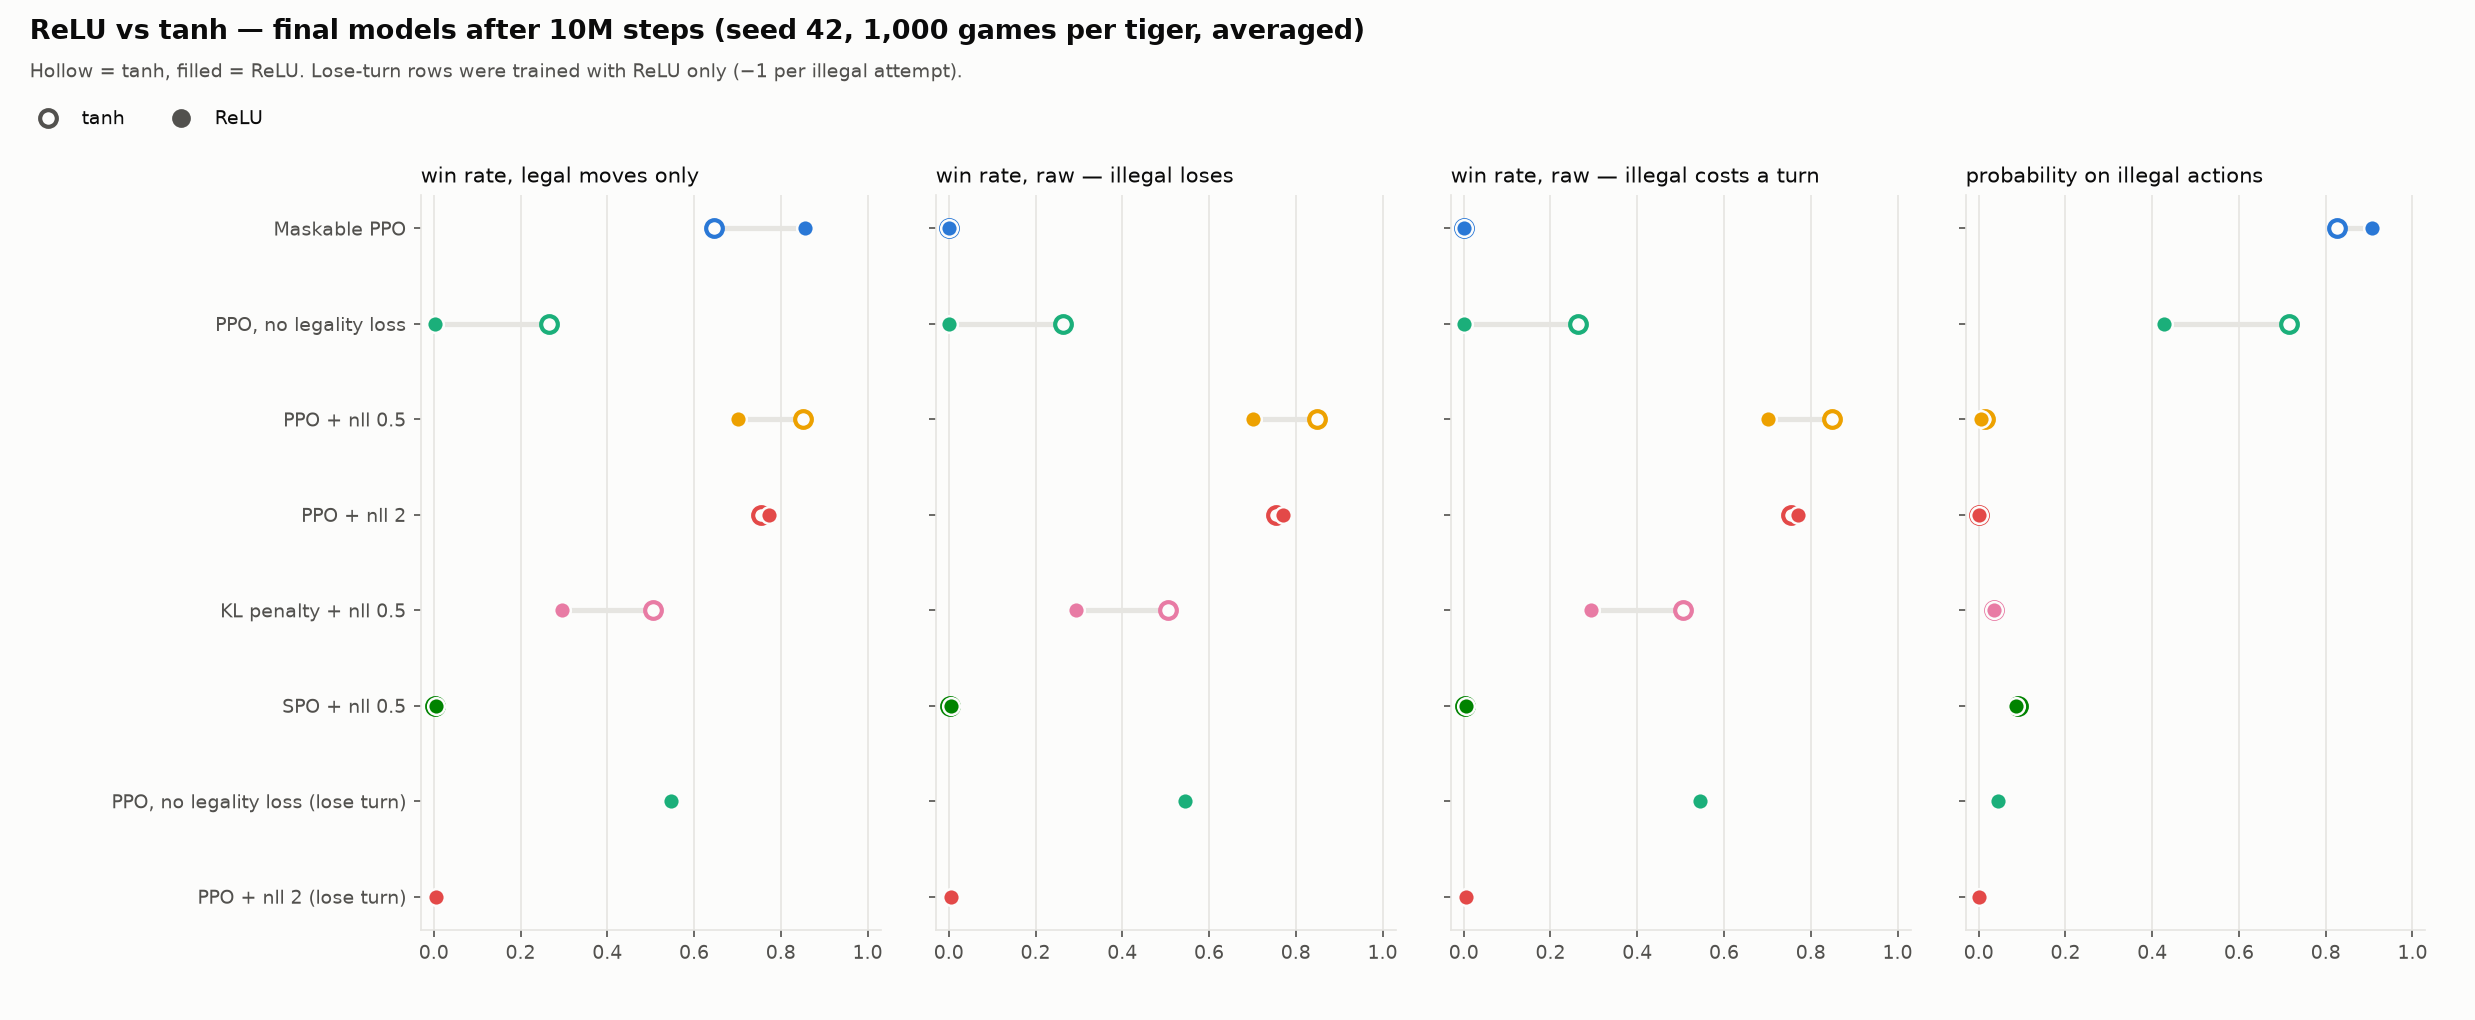
\includegraphics[width=0.8\linewidth]{figures/4_relu_vs_tanh.png}
\caption{ReLU against tanh, final models.}\label{fig:relu}
\end{figure}

\subsection{Variance of the invalid-action probability for the best model}\label{old:9.5}

Model: PPO + nll 0.5, tanh, seed 42. It played the 2,000 games of \S\ref{old:7} (1,000 per tiger) on its own: raw, argmax, an illegal move ends the game. At every decision we record $p_t = 1 - P_{\mathcal{L}}(s_t)$. Both sides are summed directly from float64 log-probabilities, so values down to about $10^{-9}$ are exact.

{\footnotesize
\begin{longtable}{@{}lrrrrrrrr@{}}
\toprule
\textbf{Decisions} & \textbf{$n$} & \textbf{mean $\bar p$} & \textbf{variance $\operatorname{Var}(p)$} & \textbf{std} & \textbf{median} & \textbf{95th pct} & \textbf{99th pct} & \textbf{max} \\
\midrule
\endhead
all & 46,810 & $4.23\times10^{-3}$ & $1.14\times10^{-3}$ & 0.034 & $4.0\times10^{-5}$ & $8.3\times10^{-3}$ & 0.094 & 0.995 \\
placement phase & 29,873 & $9.9\times10^{-4}$ & $1.27\times10^{-4}$ & 0.011 & $2.9\times10^{-5}$ & $2.5\times10^{-3}$ & 0.015 & 0.966 \\
movement phase & 16,937 & $9.95\times10^{-3}$ & $2.87\times10^{-3}$ & 0.054 & $7.6\times10^{-5}$ & 0.036 & 0.261 & 0.995 \\
vs greedy & 18,328 & $9.56\times10^{-3}$ & $2.79\times10^{-3}$ & 0.053 & $5.9\times10^{-5}$ & 0.031 & 0.254 & 0.995 \\
vs greedy, movement & 3,455 & 0.044 & 0.0123 & 0.111 & $4.4\times10^{-3}$ & 0.254 & 0.613 & 0.995 \\
vs smart & 28,482 & $8.05\times10^{-4}$ & $4.30\times10^{-5}$ & 0.0066 & $3.8\times10^{-5}$ & $2.2\times10^{-3}$ & 0.012 & 0.641 \\
\bottomrule
\end{longtable}\addtocounter{table}{-1}
}

\textbf{Decomposition.} By the law of total variance over games $j$:

\[
\operatorname{Var}(p) = \underbrace{\mathbb{E}_j\big[\operatorname{Var}(p \mid j)\big]}_{9.94\times10^{-4}\ (87\%)} + \underbrace{\operatorname{Var}_j\big(\mathbb{E}[p \mid j]\big)}_{1.44\times10^{-4}\ (13\%)}
\]
Most of the spread is between moves \emph{within} a game rather than between games.

\textbf{What drives it.} The distribution is heavy-tailed: half the decisions have $p_t < 4\times10^{-5}$, but rare movement-phase positions against the greedy tiger reach $p_t > 0.25$. The illegal probability rises through the game against greedy, from about $10^{-5}$ in early placement to a median near $2\times10^{-2}$ late in the movement phase. Against smart it stays near $10^{-4}$. In deterministic play only 73 of 46,810 choices were illegal.

\textbf{If the policy sampled instead of taking the argmax}, the probability that a whole game contains no illegal move along the same positions is $\prod_t (1 - p_t)$. Its mean is 0.93 (0.88 vs greedy, 0.98 vs smart).

\begin{figure}[H]
\centering
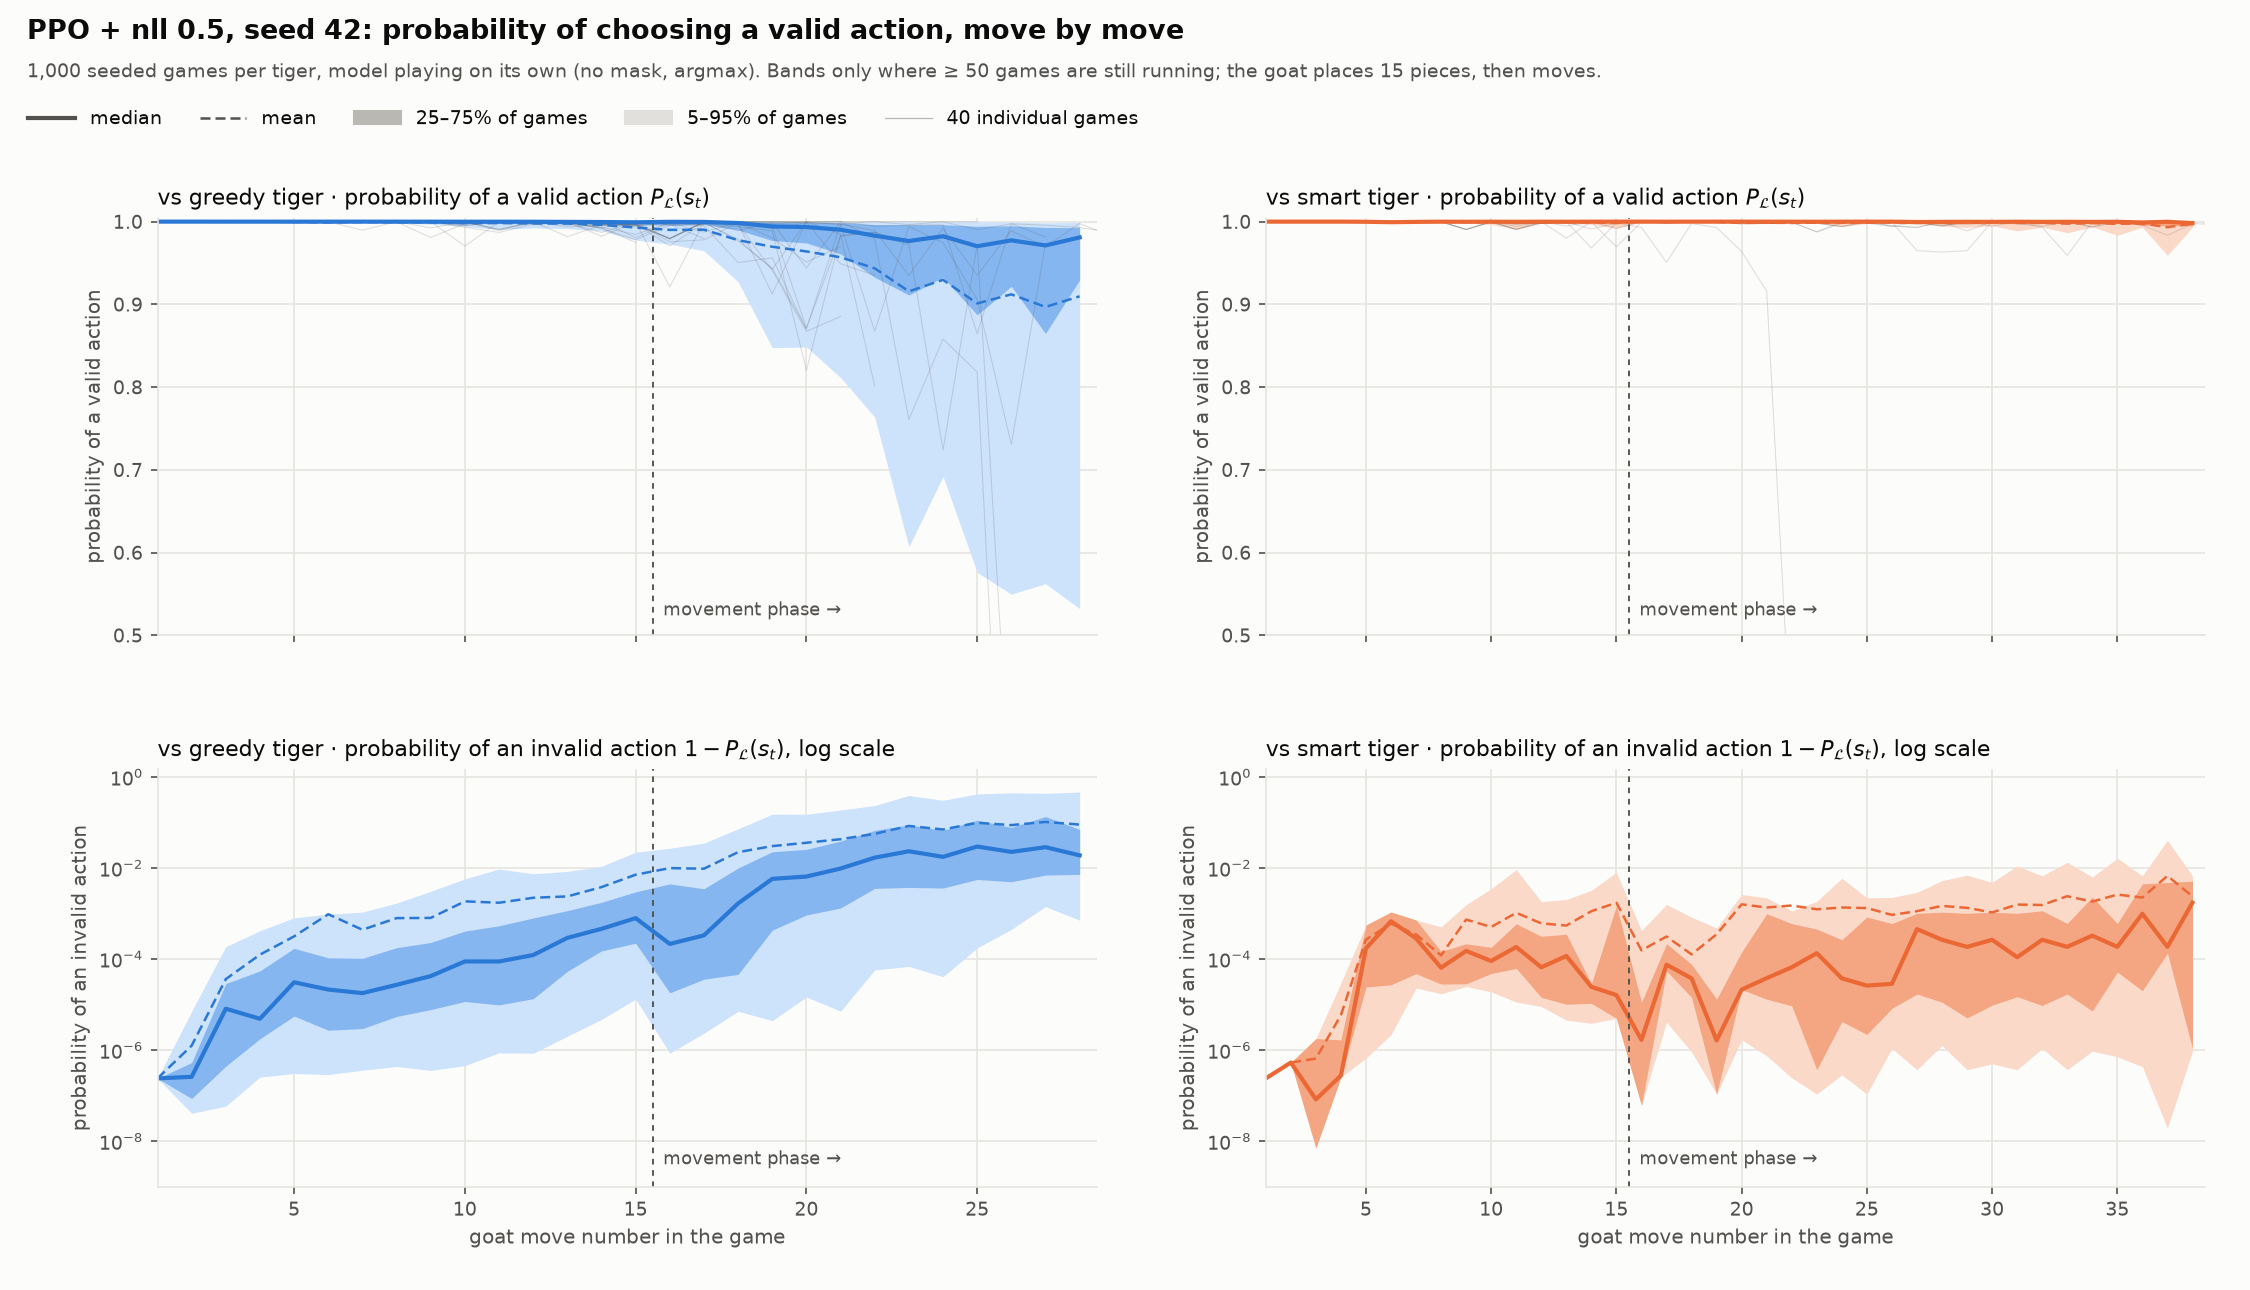
\includegraphics[width=0.98\linewidth]{figures/5_valid_probability_by_move.png}
\caption{Probability of a legal move by move number for the best model (PPO + nll 0.5, seed 42).}\label{fig:validprob}
\end{figure}

\begin{figure}[H]
\centering
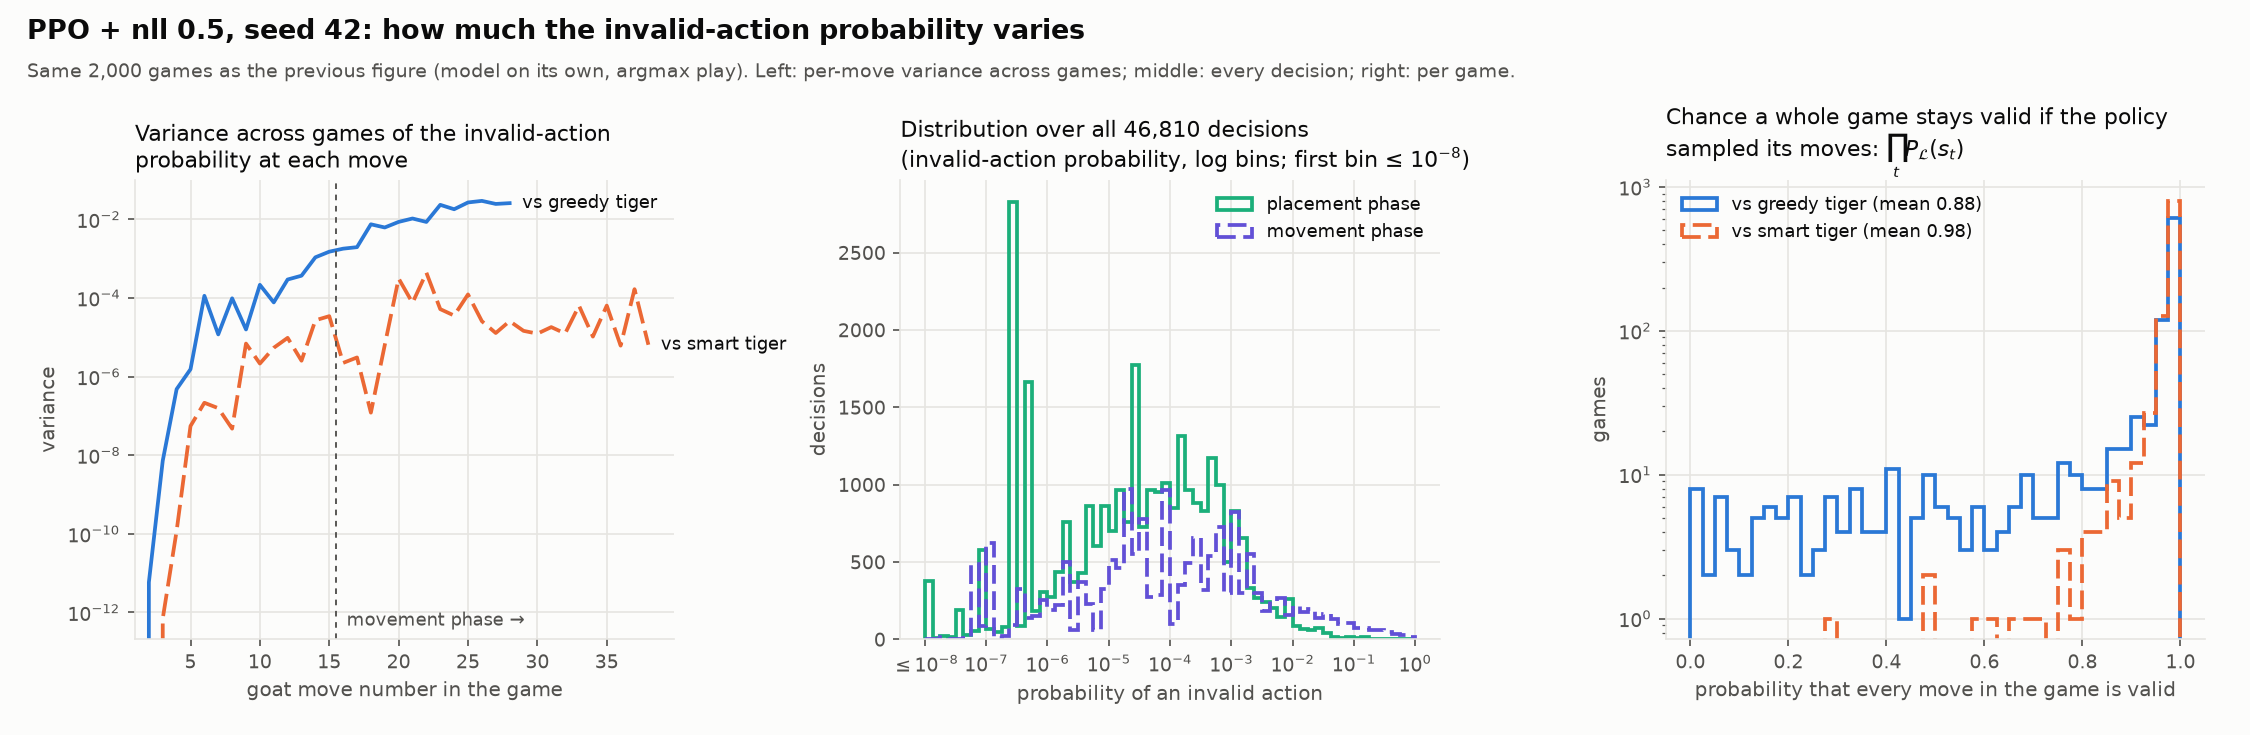
\includegraphics[width=0.98\linewidth]{figures/6_invalid_probability_variance.png}
\caption{Distribution and variance of the invalid-action probability for the same model.}\label{fig:variance}
\end{figure}
